\chapter{Internet das Coisas}
\label{cap:internet_of_things}
%%%%%%%%   PARTE 1   %%%%%%%%
%\section{Conceito}

% TODO: INTRODUÇÃO

% Contextualização

% REVER
A tecnologia, com o passar dos anos, se faz mais presente na indústria \cite{Fernandes2013}, comércio \cite{Carmona2014}, agricultura \cite{Quadros2011} etc., ao mesmo tempo tornando-se indispensável para todas essas entidades. No entanto, um novo paradigma está emergindo: a Internet das Coisas. A partir dela, a Internet vai deixar de existir como é vista hoje.

% O que é 

O conceito de Internet das Coisas (IoT) está relacionado à interconexão de objetos distintos através de uma rede, sendo esta, muitas vezes, a Internet. Desse modo, elementos do mundo real, que até então funcionavam de maneira independente ao meio em que estavam inseridos, são capazes de interagir com outros objetos à sua volta e, assim, trocar informações que possam ser relevantes. Desse modo, permite-se a agregação de novas funcionalidades.  Além disso, a IoT abre espaço para interação entre o mundo físico e o digital a partir de dispositivos capazes de capturar dados físicos no meio em que estão tais como, temperatura, distância etc., representá-los digitalmente e trasmití-los para outros dispositivos \cite{Suresh2014}.

O termo ``Internet das Coisas'' foi citado pela primeira vez por Kevin Ashton, diretor executivo da AutoIDCentre do MIT, em 1999 enquanto realizava uma apresentação para promover a ideia do uso de Identificadores de Radio Frequência (RFID) na etiquetagem de produtos. O uso da tecnologia beneficiaria a logística da cadeia de produção \cite{Finep2015}. Apesar de o termo IoT ter sido usado apenas em 1999, aplicações práticas da ideia já existiam anos antes. Um exemplo disso, é a torradeira que podia ser ligada e desligada via internet criada em 1990 \cite{Suresh2014}.

A Internet das Coisas está em grande expansão. Estima-se que, em 2020, cerca de 24 bilhões de dispositivos IoT estejam conectados, implicando em cerca de quatro dispositivos por pessoa. Para tanto, em torno de 6 trilhões de dólares serão investidos em desenvolvimento de tecnologias de hardware e software, como aplicações, segurança e dispositivos de hardware. Apesar da grande quantia investida, o setor é visto como promissor. Estima-se será gerado em torno de 13 trilhões de dólares em 2025 \cite{Meola2016}.

\section{Arquitetura}
% Escrever sobre as diversas arquiteturas existentes, características de cada uma, as melhores aplicações de cada uma etc.

Segundo \citeonline{Al-Fuqaha2015}, para que seja possível a Internet das Coisas, em meio ao grande número de objetos, são necessários seis elementos básicos: identificação de cada dispositivo na rede, sensoriamento sobre o ambiente, comunicação entre os dispositivos e a Internet, computação, serviços e semântica. As arquiteturas para Internet das Coisas, devem levar em conta esses pontos.

Com o tempo, alguns modelos de arquiteturas em camadas foram propostos no âmbito da Internet das Coisas. \citeonline{Al-Fuqaha2015} mostra algumas das arquiteturas mais comuns para IoT, entre elas, as que estão mostradas na Figura \ref{fig:cap2_arquiteturas}.
\begin{figure}[htb]
	\caption{Arquiteturas para IoT}
	\subfigure[\label{fig:cap2_arq_3layer}][3 camadas]{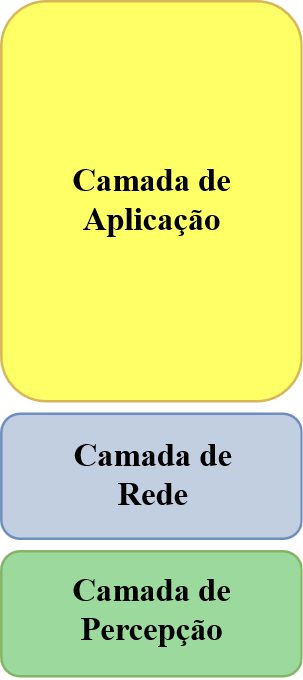
\includegraphics[width=0.25\textwidth]{cap2_arq_3layers_readaptation.png}}
	\subfigure[5 camadas]{\label{fig:cap2_arq_5layer}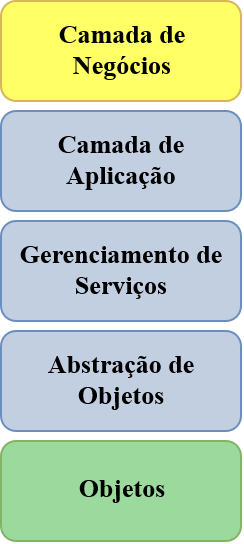
\includegraphics[width=0.25\textwidth]{cap2_arq_5layers_readaptation.png}}

	\footnotesize{Fonte: Adaptado de \citeonline{Al-Fuqaha2015}}
	\label{fig:cap2_arquiteturas}
\end{figure}

A arquitetura em três camadas pode ser definida como a base para dispositivos relacionados à IoT e envolve a  percepção, a rede e a aplicação. A primeira camada compreende os objetos inteligentes responsáveis pelo sensoriamento e a atuação sobre o ambiente, já a segunda se refere a infraestrutura de comunicação responsável por conectar os dispositivos entre si e com a Internet. Por fim, a camada de aplicação provê serviços, processamento e tomada de decisão.  

% Teoricamente

Na Figura 2.1\subref{fig:cap2_arq_5layer}, tem-se a arquitetura de cinco camadas, sendo que a primeira representa objetos dotados de sensoriamento e/ou atuação, aos quais, interagem diretamente com o ambiente. Já a segunda camada, é responsável por transmitir de forma segura os dados provenientes da camada anterior. A camada de gerenciamento de serviços atua como intermediária entre requisitores de serviços e provedores, além de processar os dados da camada inferior e entregar  serviços de acordo com o necessário. O quarto nível interage diretamente com os usuários a partir da disponibilização de serviços como exibição de informações de sensoriamento, além do controle sobre atuadores. Já a última camada é responsável por gerenciar todas as atividades e serviços da IoT, além de possibilitar a tomada de decisão e análise de \textit{big data} a partir dos dados provenientes da camada de aplicação \cite{Al-Fuqaha2015}.

% As demais arquiteturas seguem o mesmo raciocínio da arquitetura de três camadas, ou seja, um conjunto de camadas de sensoriamento, outro de infraestrutura de rede e um último de aplicação, variando em aspectos internos de cada camada de acordo com o objetivo final \cite{Ray2016}.

% Falar sobre a inexistência de um padrão global para a IoT, mas mostrar as instituições que estão tentando tornar a IoT padronizada em realidade.

\section{Tecnologias}

% Escrever sobre as tecnologias
% Introduzir comos as tecnologias influem e são necessárias na IoT.
% Contextualizar um pouco a evolução da tecnologia
% =========================================================

Para compreender melhor o funcionamento e a evolução da Internet das Coisas, é importante ter conhecimento e entendimento das tecnologias que dão base à ela. As principais tecnologias necessárias estão imersas nas camadas das arquiteturas expostas na seção anterior, ou seja, sensoriamento e atuação, redes e aplicação. A seguir, uma breve introdução em algumas das tecnologias é exposta.

\subsection{Bluetooth}

% O que é
% MELHORAR e referenciar
O Bluetooth é uma especificação de rede  \criarSigla[Rede Sem Fio de Área Pessoal]{Wireless Personal Area Network}{WPAN}, ou seja, rede sem-fio pessoal, sendo descrito e especificado pelo padrão definido pela  \criarSigla[Instituto de Engenheiros Eletricistas e Eletrônicos]{Institute of Electrical and Electronics Engineers}{IEEE}, o IEEE 802.15.1. O Bluetooth foi criado na década de 90 com o objetivo de unir tecnologias distintas, tais como computadores, celulares entre outros, a partir de uma padronização de comunicação sem fio entre os dispositivos \cite{Kardach2008}. 
%\begin{figure}[H]
%	\centering
%	\caption[ABC]{Interconexão entre diversas classes de dispositivos}
%	\label{key}
%	\includegraphics[width=0.7\textwidth]{img/bluetooth-ecosystem}
%    \newline Fonte: Repositório de imagens Pixabay %(link: 
%    %https://pixabay.com/en/bluetooth-connectivity-wireless-1690677/)
%\end{figure}
Uma das principais características dessa tecnologia \textit{wireless} é o curto alcance de transmissão variando de centímetros até alguns metros \cite{Huang2007}. 

%A tecnologia vem sendo usada ao longo dos últimos anos em diversas aplicações como transferência de arquivos entre dispositivos, transmissão de áudio entre smartphones e fones sem fio, dispositivos capazes de determinar contexto, como os beacons, entre outros.

% Topologias
No IEEE 802.15.1 há suporte para criação de redes \textit{ad-hoc}, aos quais, é desnecessário uma infraestrutura de rede para conexão dos dispositivos. A partir disso é possível criar redes chamadas \textit{picorredes}, nas quais os dispositivos são organizados em até oito associados, sendo um deles um mestre, ao qual coordena as operações, e os demais escravos \cite{BluetoothSIG2017}.

% Características
A tecnologia Bluetooth opera na \criarSigla[Industrial Científico e Médico]{Industrial Scientific and Medical}{ISM} de 2.4 GHz de uso livre em modo \criarSigla[Multiplexação por Divisão de Tempo]{Time-Division Multiplexing}{TDM} com um delta de $625\mu$s, proporcionando uma taxa de transmissão máxima em torno de 2 Mb/s, podendo variar de acordo com o dispositivo e a categoria de tecnologia de Bluetooth utilizada \cite{BluetoothSIG2017}.

% Forma de conexão.

\subsubsection{Categorias}

Segundo \citeauthor{BluetoothSIG2017}, o Bluetooth pode ser categorizado em:

\begin{enumerate}[label=(\Alph*)]
    
    \item {\criarSigla[Taxa Básica / Taxa de Dados Aprimorada]{Basic Rate/Enhanced Data Rate}{BR/EDR}}
    %2.0 a 2.1
    
    % REVER
    Esta é a subdivisão mais popularizada do Bluetooth presente nas versões $2.0$ e $2.1$, onde as principais características são alta velocidade de transmissão, baixo alcance e necessidade de conexão através da confirmação dos dispositivos. A partir disso, há um transmissão contínua de dados. Uma desvantagem é o consumo de energia considerável para o funcionamento na categoria, já que há uma conexão contínua e uma taxa de transmissão que mantêm o dispositivo ativo por um longo período ininterrupto.
    % taxa de dados
    A taxa de transmissão gira em torno de 2Mb/s.
     
    
    \item \criarSigla[Bluetooth de Baixo Consumo Energético]{Bluetooth Low Energy}{BLE}
    
    % 4.0, 4.1, 4.2
    
    % O que é
    O BLE é a mais recente categoria do Bluetooth incorporada na versão 4.0, em 2011, sendo esta a menos comum \cite{LinkLabs2015}.
    % Foco
    BLE está centrado no baixo consumo de energia para permitir que certos dispositivos não precisem recarregar ou trocar suas fontes de energia, geralmemente baterias, por longos períodos, que podem chegar a anos. 
    % Pareamento
    Para uma conexão para transmissão de dados, ao contrário do BR/EDR, não é necessário um pareamento, além disso esta tem curta duração, na ordem de milissegundos.
    %Taxa e alcance
    Ademais, a taxa de dados é baixa e o alcance alto. A baixa taxa de dados decorre do modo de funcionamento dos dispositivos BLE, aos quais, enviam dados em rajadas, ou seja, de tempos em tempos dados são transmitidos em forma de \textit{broadcast} e os dispositivos que estiverem próximos receberão esses dados. Nos intervalos de tempo em que o dispositivo não transmite, ele ``dorme'', isto é, entra em modo de consumo mínimo a fim de poupar energia.
    
    %Aplicação
    A aplicação prática dessas características está na IoT através de \textit{beacons} e \textit{wearables}, aos quais incorporam o BLE. Os beacons foram introduzidos pela \textit{Apple} em conjunto com o iOS 7, com o nome de \textit{iBeacon}, que permitia aos aplicativos possuir senso de localização \cite{Apple2014}. Com esses dispositivos é possível aprimorar a experiência do usuário em estabelecimentos como museus, supermercados, shoppings, estádios, através da identificação de contexto, uma aplicação móvel em um smartphone de um usuário pode exibir conteúdos, indicar promoções entre outros relacionados aquele dispositivo BLE.
    %
    %\begin{figure}[H]
    %	\centering
    %	\caption[ABC]{{\noindent Alguns exemplares de beacons}}
    %	\label{fig:beacons}
    %	\includegraphics[width=0.5\textwidth]{img/beacons.jpg}
    %	\newline Fonte: Shine Solutions %(link: 
    %%https://shinesolutions.com/2014/02/17/the-beacon-experiments-low-energy-bluetooth-devices-in-action/
    %\end{figure}
    
    \item{Dual-mode}
    
    Esta categoria se refere a dispositivos, como \textit{smartphones} que precisam se conectar tanto com dispositivos BR/EDR e BLE \cite{BluetoothSIG2017a}.

\end{enumerate}


\subsubsection{Bluetooth 5.0}

A versão 5.0 do Bluetooth foi lançada em dezembro de 2016 e trás consigo aprimoramentos em desempenho e segurança, garantindo duas vezes mais velocidade, quatro vezes mais alcance, oito vezes mais taxa de dados e, por fim, maior coexistência \cite{BluetoothSIG2017b}. 

Com a nova versão, veio a flexibilidade para construção de soluções baseadas em necessidade. Parâmetros como alcance, velocidade e segurança podem ser regulados para diversos objetivos a depender das aplicações \cite{BluetoothSIG2017b}.

%Algumas atualizações contribuem para a redução de interferência com outras tecnologias sem fio, dessa forma, proporciona melhor coexistência entre dispositivos Bluetooth e de outras tecnologias, dentro do cenário emergente da IoT \cite{BluetoothSIG2017b}.


% ==================================================================================================
\subsection{RFID}

O protocolo de \criarSigla[Identificação por Rádio Frequência]{Radio-Frequency IDentification}{RFID} é uma tecnologia de identificação automática, entre diversas outras como código de barras, no entanto se distingue pelo modo de funcionamento, ou seja, por ondas eletromagnéticas. Além disso, o RFID se destaca em relação às outras tecnologias no que se refere às influências externas no seu funcionamento, como sujeira, posição de leitura. Desse modo, não é necessário nem limpar ou reposicionar o dispositivo RFID para efetuar a leitura \cite{Finkenzeller2010}. 

% LEITOR E TRANSPONDER
No RFID, os dados são transmitidos através de ondas de rádio entre dois dispositivos: \textit{transponder} ou \textit{tag} e \textit{leitor}. O transponder é localizado no objeto identificado, um produto, equipamento etc., e nele são mantidos os dados de identificação. Já o leitor é responsável pela leitura e escrita destes \cite{Finkenzeller2010}.
% FUNCIONAMENTO
Para a transmissão dos dados entre os dois dispositivos o leitor emite ondas de rádio na tag. Ao receber o estímulo, a tag responde com seus respectivos dados. Além disso, existem tags que utilizam a energia do campo eletromagnético gerado pelo leitor para seu funcionamento, sendos estas chamadas de \textit{passivas}. Existem, também, aquelas que possuem uma fonte própria de energia e por isso são denominadas \textit{ativas} \cite{Finkenzeller2010}.

%Um exemplo de tag ativa é mostrada na Figura Y.

%\begin{figure}[H]
%	\centering
%	\caption[ABC]{{\noindent Exemplo tag RFID ativa}}
%	\label{fig:active-rfid}
%	\includegraphics[width=0.3\textwidth]{img/active-tag.jpg}
%	\newline Fonte: Vnsky %(link: 
%	%http://www.vnsky.com/parts/2673180/ACTIVE-TAG-REFERENCE-DESIGN-KIT.html
%\end{figure}

%Uma tag passiva é mostrada na Figura Y.

%\begin{figure}[H]
%	\centering
%	\caption[ABC]{{\noindent Exemplo tag RFID passiva}}
%	\label{fig:passive-rfid}
%	\includegraphics[width=0.3\textwidth]{img/passive.png}
%	\newline Fonte: Eletrosome %(link: 
%	%https://electrosome.com/rfid-radio-frequency-identification/
%\end{figure}

% TIPOS (alimentação)

% ATIVO
% PASSIVO

% FREQ. DE OPERAÇÃO
Uma das características mais importantes dos dispositivos RFID é a frequência de operação.
%já que ela influi no distância máxima de operação. Tal fator é determinado pelo leitor.
Os dispositivos são classificados, de acordo com esse parâmetro, em três grupos:

\begin{itemize} \parskip -3pt
	\item \textbf{Baixa Frequência (LF):} Entre 30kHz à 300kHz
	\item \textbf{Alta Frequência (HF):} Entre 3MHz à 30MHz
	\item \textbf{Ultra Alta Frequência (UHF)}: Entre 300MHz a 3GHz.
\end{itemize}

É possível distinguir pelo alcance:

\begin{itemize} \parskip -3pt
	\item \textbf{Longo alcance:} maior que um metro
	\item \textbf{Ligação remota:} até um metro
	\item \textbf{Ligação próxima:} até um centímetro
\end{itemize}

%TODO: Escrever sobre os fatores que influenciam no funcionamento, alcance etc.

% ==================================================================================================
\subsection{NFC}
% O_QUE É
O \criarSigla[Comunicação por Campo de Proximidade]{Near Field Communication}{NFC} é um sistema de comunicação sem fio derivado do RFID. Ele permite transações simples e seguras entre dois dispositivos a partir da curta distância de operação, em torno de quatro centímetros, e do funcionamento baseado em aproximação dos objetos em questão \cite{NFCForum2016}. 
Assim, é possível realizar leituras de etiquetas (do inglês, \textit{tags}) e obter conteúdos de acordo com a aplicação, transferir dados entre smartphones entre outras funcionalidades.
% COMPATIBILIDADE
Outra vantagem do NFC é a compatibilidade com a infraestrutura de cartões sem contato existentes permitindo usar um único dispositivo em tecnologias diferentes. Desse modo, é possível interagir com tags RFID, por exemplo.


% FUNCIONAMENTO
Como o RFID, o NFC funciona através de ondas eletromagnéticas, mas com uma taxa de transmissão máxima de 424 kbps \cite{NFCForum2016}. Assim como no RFID, é possível que os dispositivos NFC que contenham os dados usem a energia do leitor para transmitir seus dados, no modo passivo, ou usem uma fonte própria para tal procedimento, no modo ativo \cite{Igoe2014}.


% MODOS DE OPERAÇÃO
Outra característica importante no NFC são os modos de operação. De acordo com \citeonline{NFCForum2016} existem três modos:

\begin{itemize} \parskip -1pt
	\item \textbf{Leitor/Escritor de \textit{tag}}: Tem por objetivo ligar o mundo físico ao digital através 	de aplicações que leem e/ou escrevem em tags para obter dados e, assim, fornecer conteúdo ao 	usuário relacionado à etiqueta lida. Um exemplo é um smartphone ao ler uma tag NFC de um cartaz na 	rua.
	\item \textbf{Peer to Peer}: Visa conectar dispositivos por aproximação física e permite transferência de dados. Um exemplo é o Android \textsuperscript{\textregistered}\footnote{https://www.android.com/intl/pt-BR\_br/} Beam que possibilita a troca de arquivos entre smartphones com o 
	sistema operacional móvel da Google\textsuperscript{\textregistered}\footnote{https://www.google.com}.
	\item \textbf{Emulação de cartão}: Conecta o dispositivo do usuário em uma infraestrutura 	possibilitando a simulação de um cartão, além da realização de transações financeiras e identificação no sistema de transporte a partir da aproximação do dispositivo a um leitor 	específico.
\end{itemize}

% CATEGORIAS
Há quatros tipos de tags definidas \cite{NFCForum2016a}, sendo que todos operam no modo Leitor/Escritor descrito anteriorente : 

\begin{itemize} \parskip -1pt
	\item \textbf{Tipo 1}: 96 bytes de memória disponível e expansível para 2kiB. Usuário pode 
	configurá-la para somente leitura.
	\item \textbf{Tipo 2}: 48 bytes de memória disponível e expansível para 2kiB. Usuário pode 
	configurá-la para somente leitura.
	\item \textbf{Tipo 3}: Baseado no padrão industrial japonês e conhecido como FeliCa. Pode ser 
	configuradas para leitura/escrita ou somente leitura na fabricação. A memória disponível varia, 
	mas com um limite teórico de 1MiB.
	\item \textbf{Tipo 4}: A memória disponível varia estando acima de 35 kiB por serviço. É 
	possível ser configurada para leitura/escrita ou somente leitura.
\end{itemize}

O NFC possui um padrão com o qual dispositivos devem estar formatados, o \criarSigla[Formato de Troca de Dados por NFC]{NFC Data Exchange Format}{NDEF} (\textit{NFC Data Exchange Format}) um formato comum de comunicação \cite{Igoe2014}. Desse 
modo, os dados armazenados em tags devem estar gravados nesse formato. A partir do NDEF é possível armazenar e trocar documentos binários como Mime, que incluem imagens, arquivos \criarSigla[Formato de Documento Portável]{Portable Document Format}{PDF} entre outros, 
\criarSigla[Localização Uniforme de Recursos]{Uniform Resource Locator}{URL}, texto simples entre outros.


% ==================================================================================================
\subsection{Zigbee}

% WHAT IS IT
O Zigbee é um protocolo padrão de comunicação de baixa potência para redes sem-fio \textit{mesh}, ao qual permite a diversos dispositivo trabalharem em conjunto \cite{Faludi2011}. Além disso, é descrito como um conjunto de camadas implementadas sobre o IEEE 802.15.4 \cite{Faludi2011}, ao qual especifica a camada física (PHY) e o controle de acesso ao meio (MAC) para redes sem-fio de baixa potência (WLAN) \cite{IEEE2011}.

As camadas do Zigbee, de acordo com \citeonline{Faludi2011}, responsabilizam-se pelo:

\begin{itemize} \parskip -4pt
	\item \textbf{Roteamento:} Tabelas de roteamento que definem como um nó envia dados até um 
	destino.
	\item \textbf{Rede Adhoc:} Criação automática de rede.
	\item \textbf{Malha Auto-Curativa (do inglês, \textit{Self healing mesh}):} Descobe se nós se perderam da rede e a 
	reconfigura para garantir uma rota para os dispositivos conectados ao nó faltantes.
\end{itemize}

O Zigbee opera na faixa não licenciada ISM, de 2,4GHz, o que permite sua expansão global e, assim, ter a capacidade de operar em qualquer local do mundo. Além disso, especifica que os nós das redes criadas possam assumir papeis específicos \cite{Faludi2011}, sendo eles:

\begin{itemize} \parskip -4pt
	\item \textbf{Coordenador}: Responsável por criar a rede, distribuir endereços, manter a rede segura e em funcionamento entre outras funções. Cada rede tem um e apenas um coordenador.
	\item \textbf{Roteador}: Tem capacidade de unir redes existentes, enviar e receber informações e rotear 	informações, atuando como um intermediário entre dispositivos. É permitido às redes terem múltiplos roteadores, bem como possuírem nenhum. No entanto no caso de existirem, cada roteador deve estar conectado a um coordenador ou outro roteador.
	\item \textbf{Dispositivo final}: É um tipo de nó capaz de se unir a redes e de enviar e receber informações da rede. Além disso, podem se desligar de tempos em tempos para poupar energia. Caso mensagens para um dispositivo final desligado sejam detectadas, o nó responsável por ele,	podendo ser um coordenador ou roteador, armazena as mensagens até que o nó desperte.
\end{itemize}

Há diversas topologias suportadas, nas quais, englobam os três tipos de nós e suas possíveis 
maneiras de organização \cite{Faludi2011}:

\begin{itemize} \parskip -4pt
	\item \textbf{Par a par}: Uma rede formada apenas por dois nós, sendo um deles, obrigatoriamente, um 
	coordenador e nó restante podendo ser um roteador ou dispositivo final.
	\item \textbf{Estrela}: Nessa topologia, o coordenador se situa no centro da rede e os demais nós, 
	roteadores ou dispositivos finais, conectados apenas a ele, formando uma rede no formato de 
	estrela.
	\item \textbf{Malha (do inglês, \textit{Mesh})}: Os dispositivos finais circundam os demais nós roteadores e coordenador. O coordenador e roteadores atuam como intermediários, roteando mensagens para dispositivos finais, outros roteadores ou para o coordenador. Apesar da nova função do coordenador, este permanece no controle e gerenciamento da rede.
	\item \textbf{Árvore de agrupamento (do inglês, \textit{Cluster tree})}: Nessa topologia, cada roteador é responsável por um conjunto de dispositivos finais. As mensagens vindas desses dispositivos devem ser encaminhadas primeiramente para seu roteador responsável para então ser encaminhada ao destino na rede.
\end{itemize}

% TODO: Colocar ilustração das topologias

O Zigbee define três maneiras de identificação de nodos, que podem utilizadas em uma aplicação para 
diferenciar os nós.

\begin{itemize} \parskip -4pt
	\item \textbf{64 bits}: Único e permanente para cada rádio fabricado.
	\item \textbf{16 bits}: Dinamicamente configurado pelo coordenador ao entrar em uma rede. É único apenas 
	dentro do contexto da rede.
	\item \textbf{Node Id}: Pequena cadeia de texto. Não é possível garantir sua unicidade em nenhum contexto.
\end{itemize}

\subsection{Wi-Fi}
% O que é
Wi-Fi, é uma das diversas classes de \criarSigla[Rede Local Sem Fio]{Wireless Local Area Network}{WLAN} normatizado pelo padrão IEEE 802.11, no qual foca nas camadas física e de enlace do modelo \criarSigla[Conexão de Sistema Aberta]{Open System Interconnection}{OSI} \cite{Gast2005}. 
Além disso, há padrões específicos para o Wi-fi, como o 802.11a, 802.11b e 802.11g,  além da possibilidade de unir alguns de padrões para formar outros híbridos, como o 802.11a/g e 802.11a/b/g \cite{Kurose2012}. 

Apesar da distinção, os padrões citados compartilham diversas características, como o protocolo de acesso ao meio, estrutura de quadros da camada de enlace, habilidade de reduzir a taxa de transmissão a fim de alcançar distâncias maiores. A principal diferença é vinculada à camada física.

Os padrões a, b e g são regulamentados de acordo com a Tabela \ref{tab:ieee80211abg-phy}, sendo que pode variar em diversos países.

\begin{table}[hbt]
    \caption{Resumo dos protocolos 802.11}
    \label{tab:ieee80211abg-phy}
    \centering
    \begin{tabular}{@{}ccc@{}}
        \toprule
        \textbf{Padrão} & \textbf{Faixa de Frequências} & \textbf{Taxa de dados} \\ \midrule
        802.11b         & 2,4 - 2,485 GHz               & até 11 Mbps            \\
        802.11a         & 5,1 - 5,8 GHz                 & até 54 Mbps            \\
        802.11g         & 2,4 - 2,485 GHz               & até 54 Mbps            \\ \bottomrule 
        \end{tabular}
        
    Adaptado de: \citeonline{Kurose2012}
\end{table}



Além dos três protocolos citados há outros mais recentes ou que estão em fase de criação. O protocolo 802.11n, por exemplo, criado em 2012, faz uso de múltiplas antenas e, além disso, permite atingir uma taxa de transmissão de centenas de megabits por segundo. \cite{Kurose2012}.

A arquitetura básica do IEEE 802.11, exposta na \reffig{cap2_arquitetura-ieee80211},  é formada por \criarSigla[Conjunto Básicos de Serviço]{Basic Service Set}{BSS} onde cada um é composto de um Ponto de Acesso (AP), um dispositivo para unir os conjuntos, sendo esse um roteador ou \textit{switch}, responsável por ligar cada BSS à Internet e, por fim, os dispositivos que desejam se conectar a rede.

\figura{cap2_arquitetura-ieee80211}{Arquitetura básica para o IEEE802.11}{0.6\textwidth}{Kurose2012}


% Taxonomia
    % Adhoc
    % 
O IEEE 802.11 suporta dois tipos de interconexão de dispositivos: \textit{ad-hoc} e ponto de acesso com dispositivo. No primeiro caso, é possível interconectar dispositivos, como notebooks, sem a necessidade de uma infraestrutura de rede, no entanto com a impossibilidade de conexão com a Internet. Assim, é possível efetuar transferência de arquivos de maneira rápida e sem cabos. Além de redes ad-hoc, suporta conexões entre um ponto de acesso e um dispositivo para conexão com a Internet. Em diversos casos, o AP e o roteador estarão incorporados em um mesmo dispositivo \cite{Kurose2012}.

% Mobilidade

%O protocolo permite a mobilidade de um dispositivo entre pontos de acessos e ainda assim manter a conexão com estes sem a necessidade de se obter um novo endereço IP. Isso será possível se ambos os pontos de acessos fizerem parte de uma mesma subrede.

% Tipos de escaneamento numa mesma subrede
Existem algumas funcionalidades mais avançadas no IEEE 802.11. Uma delas se refere à possibilidade de se adaptar a taxa de dados a partir da escolha da técnica de modulação da camada física de acordo com as características do canal. Há também a possibilidade de reduzir o consumo de energia fazendo com que o nó permaneça em modo \textit{sleep} por determinados períodos de tempo o que pode gerar uma economia de até 99\% \cite{Kurose2012}.

No contexto da Internet das Coisas, o Wi-fi é fundamental na inserção de novos dispositivos à Internet. O seu uso propiciará o crescimento destes sem a necessidade da expansão da infraestrutura a cada novo objeto conectado \cite{Suresh2014}.

\subsection{Outros}
% Z-wave
Entre as tecnologias utilizadas em Smart Homes está o Z-Wave, um protocolo sem fio focado em automação residencial e comercial de pequeno porte, criado pelo ZenSys e hoje representado pela Z-Wave Alliance  \cite{Gomez2010}. O protocolo foi desenvolvido especificamente para controle, monitoramento e verificação de estado. Em relação a aspectos técnicos, o Z-Wave opera na faixa de frequências em torno de 1GHz, o que evita interferências com outras tecnologias como Bluetooth e Wi-Fi que operam em 2,4GHz, em geral. Entre as principais vantagens do Z-Wave está a interoperabilidade, além da segurança obtida a partir do uso de criptografia AES128 \cite{Z-WaveAlliance2015}.
\sigla{AES}{Advanced Encryption Standard}

% 6LowPan
Por outro lado, há a tendência de dispositivos IoT conectados à Internet usarem o protocolo de endereçamento IPv6 para serem identificados na rede. No entanto, algumas das aplicações terão limitações como fonte de energia e capacidade de transferências de dados limitadas. Como proposta de solução, tem-se o 6LowPan, definido no RFC 6282 pela Internet Engineering Task Force (IETF) focado em dispositivos com restrições de consumo de energia \cite{Olsson2014}. A principal característica desse protocolo é a redução da transmissão de dados a partir da compressão dos cabeçalhos do IPv6. Com isso, o 6LowPan é capaz de reduzir a sobrecarga de pacote para dois bytes \cite{Al-Fuqaha2015}. As redes 6LoWPAN são conectadas às redes IPv6 a partir de roteadores de borda, capazes de trocar dados entre os dispositivos dentro da rede 6LoWPAN e a Internet além de ser responsáveis por manter a rede em funcionamento. Outra característica importante nesse padrão é a viabilidade de se implementar o IPv6 em redes IEEE 802.15.4 \cite{Olsson2014}.


%%%%%%%%%%%%%%%%%%%%%%%%%%%%%%%%%%%%%%%%%%%%%%%%%%%%%%%%%%%%%%%%%%%%%%%%%%%%%%%%%%%%%%%%%%%%%%%%%%%%%%%

%%%%%%%%%%%%%%%%%%%%%%%%%%%%%%%%%%%%%%%%%%%%%%%%%%%%%%%%%%%%%%%%%%%%%%%%%%%%%%%%%%%%%%%%%%%%%%%%%%%%%


\section{Ambientes inteligentes}

A Internet das Coisas trará tecnologia os mais diversos ambientes e, assim, aprimorará as funcionalidades existentes além de trazer novas. A seguir, alguns ambientes em destaque são expostos e como a Internet das Coisas atua nestes casos. 

\subsection{Smart grid}

Na rede elétrica tradicional, a inteligência, ou seja, o controle, sensoriamento etc., é concentrada nas unidades geradoras de energia e parcialmente nos distribuidores. Além disso, o fluxo de energia é unidirecional, seguindo apenas um caminho entre a geração e o consumo. No entanto, com o aumento do uso de fontes próprias geração de energia como placas fotovoltaicas em residências, além do crescimento do consumo tem-se a necessidade de adaptação do modelo de rede elétrica existente. As \textit{smart grids} surgiram, então, como modelo alternativo de geração e distribuição de energia elétrica, onde o fluxo de energia passa a ser bidirecional e o uso de tecnologias de medições de consumo permitem prever demandas, otimizar a distribuição e aprimorar a eficiência e a confiabilidade do sistema elétrico \cite{Cecilia2016}. 

%Empresas como a \textit{Texas Instruments} (TI) têm investido em soluções para smart grid que proporcionam segurança, eficiência e inteligência. A TI oferece soluções para monitoramento da rede através de medidores de eletricidade, gás e calor, além de tecnologias para comunicação como o \textit{Power Line Communications} entre outras \cite{TexasInstruments2017}.

\subsection{Smart home}

% TODO: Conceitos
O conceito de \textit{smart home} ou casa inteligente propõe um novo modelo para um ambiente domiciliar. A implementação e o uso da tecnologia nesse ambiente abrem espaço para novas formas de interação, além de proporcionar mais comodidade e um melhor gerenciamento dos equipamentos presentes. Isso será possível graças ao uso de sensores e atuadores tanto no ambiente, como nos eletrodomésticos e utensílios. E, para interconectar todos os dispositivos, será feito uso das tecnologias de rede existentes, como o Zigbee e a Internet.

A interconexão dos dispositivos em uma casa inteligente proporcionará, como descrito, funcionalidades inéditas de interação de acordo com as ações do morador, como entrar e sair de um cômodo da casa. Nesse caso, seria possível implementar um sistema que apagasse e acendesse a lâmpada conforme os sensores de presença indicarem a ausência do indivíduo e a hora do dia \cite{DeSilva2012}.

Entre as apostas para as casas inteligentes está o aumento da eficiência do consumo energético. O uso da tecnologia por meio de medidores de energia, tomadas e aparelhos inteligentes permitirá o monitoramento e controle do consumo dos dispositivos da casa. Com base nisso, é viável a otimização do consumo de cada equipamento controlando-o para ativá-lo somente quando necessário e, assim, evitar desperdícios. Além disso, é viável a previsão da demanda de energia para cada momento do dia \cite{Stojkoska2017}.

As casas inteligentes necessitam que os dispositivos sejam organizados hierarquicamente para garantir o bom desempenho dos componentes do sistema. \citeonline{Stojkoska2017} propõe um modelo, mostrado na \reffig{cap2_smart-home_framework-stojkoska} para organização de casa inteligente que integra \textit{smart grid} e envolve cinco componentes principais: a casa inteligente em si, a nuvem, unidade geradora de energia, aplicações de terceiros e interfaces de usuário. Nesse contexto, a casa inteligente contém redes de sensores sem fio que adquirem dados do ambiente e enviam esses dados para um \textit{home hub}, um ponto central capaz de se conectar à uma rede externa. Já a unidade geradora de energia é responsável por, além da geração e fornecimento de energia, trocar informações sobre custo da energia, consumo atual e futuro da casa entre outros. 
A nuvem é responsável por armazenar todos os dados provenientes de sensores e outros dispositivos da casa e por comportar uma infraestrutura de processamento. 

A partir dos dados existentes na nuvem é possível que as aplicações de terceiros entreguem soluções web ou aplicações mobile para os usuários. Para obter acesso às soluções, o último componente é necessário: a interface de usuário. Nesse ponto, o usuário tem em mãos a capacidade de monitorar em tempo real os gastos de energia dos equipamentos de sua casa, bem como controlá-los de acordo com a sua necessidade e desejo.

\figura{cap2_smart-home_framework-stojkoska}{Modelo para casas inteligentes}{\textwidth}{Stojkoska2017}

%(escanoladores, reguladores, balanceadores de carga).
%(stoj...; mostrar a figura do cara)

% Segundo \cite{DeSilva2012}, as casas inteligentes podem ser divididas em três categorias principais. 
% A primeira delas atenta-se em detectar e reconhecer ações dos moradores e seu estado de saúde e, baseando-se nelas, prover serviços com foco no bem-estar e na saúde dos residentes. Nesse categoria estão incluídos cuidado de idosos, da saúde e de crianças. 
% A segunda categoria se refere à captura e multimídia de eventos ocorridos no dia a dia.
% A terceira tem como foco na segurança. Uma sistema de alerta pode ser ativado, no momento em que uma invasão, sequestro ou desastre natural ocorrer, a partir captura de imagens, sensoriamento entre outros.


Uma casa inteligente permite que os moradores tenham maior independência no seu dia a dia, especialmente em caso de pessoas idosas, com dificuldade de locomoção, além daquelas com deficiências físicas e visuais.
No seu artigo, \citeonline{DeSilva2012} propõe um sistema que usa imagens de uma casa, capaz de detectar o dia a dia de uma pessoa idosa. É possível também identificar possíveis quedas e avisar o responsável ou o atendimento médico. Apesar, da aplicação citada possuir um enfoque no morador, não há muitas propostas para casa inteligente com o foco nos usuários, no entanto, existem muitas que focam nos aspectos técnicos, como dispositivos, arquiteturas entre outros \cite{Wilson2015}.



%Em relação às tecnologias para desenvolvimento de aplicações e dispositivos para casas inteligentes, tem-se diversos sistemas sendo implementados. Entre eles está o projeto \textit{Eclipse SmartHome} \textsuperscript{\texttrademark}
%\footnote{http://www.eclipse.org/smarthome}, ao qual disponibiliza aos desenvolvedores um \textit{framework} para desenvolvimento de soluções casas inteligentes e ambientes assistidos destinadas a usuários finais. 
    
% TODO: Desafios

A empresa \textit{Amazon} \textsuperscript{\textregistered}
\footnote{https://www.amazon.com/} oferece o \textit{Amazon Echo}, um dispositivo que dispõe de diversas funcionalidades multimídia, como reprodução de músicas através de controle por voz, além de oferecer informações como previsão do tempo, notícias, tráfego entre outros através do \textit{Alexa Voice Service} (Serviço de Voz Alexa). É capaz de controlar a luz, tomadas e termostatos além de ser compatível com produtos de empresas, como SAMSUNG\textsuperscript{\textregistered}
\footnote{http://www.samsung.com/br/}, Philips{\textregistered}
\footnote{http://www.philips.com.br/} entre outras, com foco em \textit{smart homes} \cite{amazon2017}.

%\subsubsection{Smart Kitchen}

Seguindo a lógica das casas inteligentes, as \textit{Smart Kitchens} ou cozinhas inteligentes promovem o aprimoramento dos dispositivos da cozinha com a inserção da tecnologia. A partir disso, utensílios como panelas, talheres entre outros poderão fazer uso de tecnologia para entregar novas funcionalidades \cite{Staender2012}. Por exemplo, no caso das panelas, é possível colocar sensores de temperatura e câmera para determinar a temperatura atual e o estado atual do alimento que está sendo cozido. A partir disso, o sistema computacional presente na panela, processará os dados e fará uma comunicação com o fogão para ajustar a intensidade do fogo caso ainda não esteja pronto, ou simplesmente, desligar o fogo, caso o esteja. 

\subsection{Outros}
%\subsection{Smart factory}
% Quarta revolução industrial,

% Apoio a logística

%\subsection{Smart City}

Entre os ambientes inteligentes em expansão está a cidade inteligente ou \textit{smart city}. Apesar de não ter uma definição conceitual clara \cite{Cocchia2014}, no contexto da Internet das Coisas, a ideia principal por trás desse ambiente é trazer qualidade de vida aos cidadãos, crescimento sustentável e melhor uso de recursos públicos, aos quais são possíveis graças ao uso da IoT com foco no ambiente urbano. A Internet das Coisas, nesse contexto, permite uma melhor gerenciamento, otimização dos serviços públicos como transporte, iluminação, vigilância e manutenção de áreas públicas entre outros  \cite{Zanella2014}. 

%
Já no ambiente industrial, a Internet das Coisas em conjunto com sistemas interconectados promoverá a Indústria 4.0 também chamada quarta revolução industrial. Ademais, os sistemas cyber-físicos, aos quais podem ser definidos como sistemas que integram processos físicos, computacionais, de comunicação e de rede, integrados com a Indústria 4.0, poderão ser definidos como a \textit{smart factory} ou fábrica inteligente \cite{Lee2015}. Por outro lado, a Indústria 4.0 é vista como possível solução para problemas atuais em indústrias como poluição, consumo de combustíveis fósseis entre outros \cite{Hussain2016}.

% \subsection{Wearables}

% \textit{Wearables} são dispositivos computacionais vestíveis, ou seja, são itens que uma pessoa pode usar no dia a dia como, roupas, relógios, óculos, sapatos entre outros e, ainda obter novas funcionalidades, graças à presença da tecnologia nesses dispositivos. Isso é possível devido a sensores aos quais medem sinais vitais do corpo humano e dados do ambiente, a depender da aplicação, além de pequenos equipamentos de hardware responsáveis por ler os dados dos sensores e comandos do usuário e assim tomar as ações necessárias de acordo com a situação.

% Os \textit{wearables} têm aplicações nas mais diversas áreas, partindo das áreas da saúde e esportes até lazer e trabalho. 

% Algumas empresas têm investido na área de dispositivos vestíveis. Um exemplo é a Microsoft que vem desenvolvendo o \textit{Holo Lens}, um dispositivo que se assemelha a um óculos, com foco em realidade aumentada. A tecnologia pode ser usada na concepção e design de produtos, educação, astronomia entre outros.

% Outra tecnologia em ascensão é o \textit{smart watch}, relógio digital conectado à internet, dotado de aplicativos entre outras funções que vão além de mostrar as horas.

% Na área de esportes e saúde, existem as \textit{smart bands}, pulseiras capazes de monitorar sinais, como batimentos além das calorias eliminadas durante um exercício, distância percorrida entre outros.



%\subsection{Turismo}
% Exemplo de turismo do artigo
%Uma aplicação proposta consiste em um sistema de informação turístico com intuito de expandir a experiência dos visitantes nos diversos pontos turísticos no Japão. Isso é possível graças ao uso de beacons, sensores sem fio descritos na seção anterior, e realidade aumentada, viabilizada por uma aplicação móvel \cite{SHIBATA2016}. 


\section{Desafios}

% Contextualizar
Apesar dos avanços constantes, a área de Internet das Coisas terá de superar alguns desafios para que possa se expandir sem prejudicar o desempenho das aplicações e a experiência dos usuários. Esses desafios, segundo \citeonline{Hussain2016}, são a heterogeneidade dos dispositivos, a interoperabilidade, a escalabilidade, segurança, privacidade e Qualidade de Serviço (QoS).

% Heteregeineidade
O primeiro dos desafios, a heterogeneidade, se refere as diferenças de hardware e software dos dispositivos bem como seu propósito, como objetivos, plataforma de hardware, modos de interação, entre outros. %Um solução simples à primeira vista, é fazer com que se use os mesmos padrões de hardware e software, no entanto não há uma única tecnologia de comunicação, por exemplo, que supra as necessidades de todas aplicações existentes.

% Interoparabilidade
A Interoperabilidade diz respeito à capacidade de dispositivos, que usam diferentes tecnologias, poder interagir. Nesses casos é necessário um dispositivo que atue como mediador ao qual tem acesso a ambas tecnologias para que a troca de dados ocorra.

% Escabilidade
Outro grande desafio é a escalabilidade. As aplicações de IoT devem suportar o crescimento do número de dispositivos conectados, usuários, aplicações entre outros sem qualquer comprometimento da Qualidade de Serviço (QoS). Esse aumento em dispositivos e afins, deve ser refletida nos recursos que sustentam a IoT. 
% Em meio ao grande número de dispositivos, comunicação e interligação são desafios da IoT.

% Segurança e privacidade
A segurança e privacidade, da mesma forma, requerem atenção. A restrição de recursos torna difícil proteger a informação. Ainda assim, é necessário garantir transações seguras e o não comprometimento dos dados do usuários. No entanto, os métodos tradicionais não podem ser utilizados, pois diferentes padrões estão envolvidos. Por outro lado, IoT implica em conexão global, ou seja, implica que qualquer indivíduo pode acessar externamente. 
Portanto, há a necessidade de novos mecanismo que garanta a segurança e privacidade, sendo relevante aos desenvolvedores garantir esses requisitos em suas aplicações. 


% Quality of Service
A Qualidade dos Serviços em IoT vem sendo estudado com frequência. Entre os principais desafios estão disponibilidade, confiabilidade, mobilidade, desempenho, escalabilidade entre outros. No entanto, nem toda a aplicação exige que os pontos citados sejam atendidos integralmente \cite{Hussain2016}. 